\documentclass[aps,floatfix,11pt]{revtex4-1}
\usepackage{bm}%bold math
\usepackage{graphicx}
\usepackage{amsmath}
\usepackage{amssymb}
\usepackage{setspace}
\linespread{1}

\begin{document}

\title{Notes}

\date{\today}

\begin{abstract}
    
\end{abstract}

\maketitle 

\section{Updated Moves and Rules}

\subsection{Star Pair Creation and Annihilation}

Creation and annihilation of a horizontal pair of stars is shown in fig.
\ref{fig:create_annihilate_pair}. Creation and annihilation of a vertical pair of stars can be
is simply what is shown in fig. \ref{fig:create_annihilate_pair} rotated by $\pi/2$.

\begin{figure}[h]
    \centering
    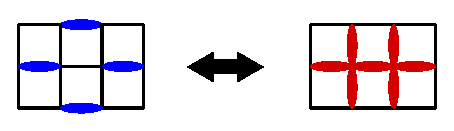
\includegraphics[width=8.5 cm]{create_annihilate_pair}
    \caption{The creation and annihilation of a pair of stars.
\label{fig:create_annihilate_pair}}
\end{figure}

\subsection{Star Horizontal/Vertical Translation}
Horizontal translations of a star is shown in fig. \ref{fig:move_right_left}. The vertical
translations can be obtained by rotating fig. \ref{fig:move_right_left} by $\pi/2$. Horizontal
translations must be preformed such that the star remains on its original sub-lattice, thus the
minimal translation is by two vertices.

\begin{figure}[h]
    \centering
    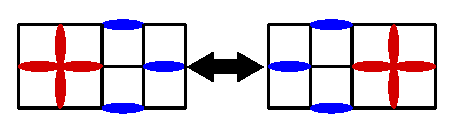
\includegraphics[width=8.5 cm]{move_right_left}
    \caption{Horizontal translation of a star.
\label{fig:move_right_left}}
\end{figure}

\subsection{Star Diagonal Translation}
A star can remain on its original sub-lattice through a diagonal translation as well. It turns out
that the diagonal translations can occur in a wider variety of cases. We show a star moving
diagonally in the upward right direction in fig. \ref{fig:diag} where there are three possible
allowed movements in this direction of this order. We see that diagonal movement can happen as long as
the following conditions are met.

\begin{itemize}
    \item of the $3\times 3$ square the furthest vertex from the star must not be the center of a
        different star.
    \item there must be two dimers occupying 2 of the 6 occupiable links in the corner furthest from
        the star. This ensures that the star is not moved into a position where it is breaking
        "number of links around a vertex" rules.
\end{itemize}

\noindent
If the above conditions are satisfied there are two possible ways to make the move for any movable
diagonal configuration (any direction). 1) Rotate the $3\times3$ square by $\pi$, 2) reflection
about the diagonal of the square that is perpendicular to the direction of movement. The second
option will flip the "not star" dimers from vertical to horizontal and visa versa. For now we only
implement the first option (rotation). Unfortunately we must distinguish between translations
happening along different diagonals. A general rotation does not suffice because we do not want to
alter, swap, or in any way change the corners of the $3\times 3$ square that are off the diagonal of
the translation.

\begin{figure}[h]
    \centering
    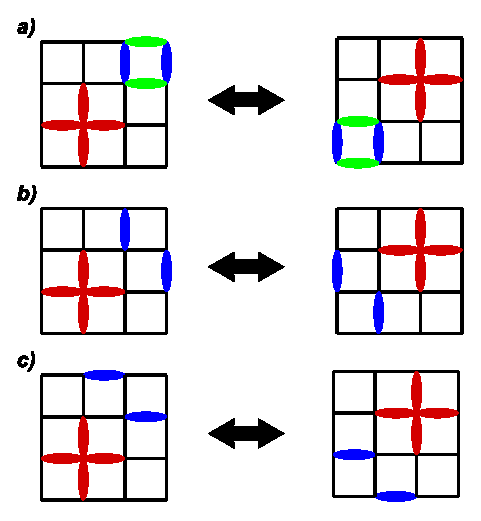
\includegraphics[width=8.5 cm]{diag}
    \caption{Diagonal translation in the upward right direction.
\label{fig:diag}}
\end{figure}


\section{Old Moves and Rules}

Creating a pair of stars in the staggered state is shown in fig. \ref{fig:old_create_pair}. We notice
the creation of a star produces two flippable plaquettes between the two stars.

\begin{figure}[h]
    \centering
    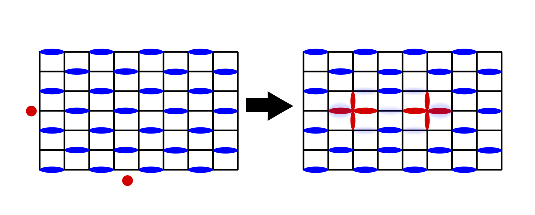
\includegraphics[width=8.5 cm]{old_create_pair}
    \caption{The creation of a pair of stars in the fully packed staggered configuration. The red
    dots on the $x$ and $y$ axes show the dimer about which the stars are created.
\label{fig:old_create_pair}}
\end{figure}

\noindent In fig. \ref{fig:old_move_right} we show the rightmost star move right in the same
configuration. In any single star must remain on the sublattice it was created on, so the center of
the star moves by two vertices. We notice that the horizontal propagation of a star creates two boundaries of
flippable plaquettes across the top and bottom of the star pair. 

\begin{figure}[h]
    \centering
    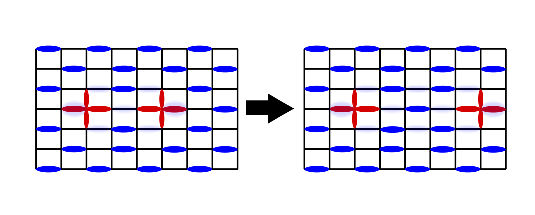
\includegraphics[width=8.5 cm]{old_move_right}
    \caption{The move of the rightmost star in fig. \ref{fig:old_create_pair} \label{fig:old_move_right}}
\end{figure}

Still figuring out the possible ways to move stars vertically. In six steps we show it is possible
to implement a specific type of local vertical move. 
\\

\begin{itemize}
    \item 
    Step 1 (fig. \ref{fig:ex_vert_mv_1}): create a pair of stars.
    
    \item 
    Step 2 (fig. \ref{fig:ex_vert_mv_2}): Move rightmost star right four times creating a horizontal set of
    flippable plaquettes.
    
    \item
    Step 3 (fig. \ref{fig:ex_vert_mv_3}): Flip some of the plaquettes. 
    
    \item
    Step 4 (fig. \ref{fig:ex_vert_mv_4}): With several vertical pairs of dimers we can flip on plaquette to make a
    horizontal pair that was not part of the original set of horizontal dimers after the star move. The
    $x$ and $y$ positions of this plaquette are marked in fig. \ref{fig:ex_vert_mv_4} by red dots along the $x$ and $y$
    axes. If all of the dimers were left as vertical or horizontal the move would not be possible.
    
    \item
    Step 5 (fig. \ref{fig:ex_vert_mv_5}): Create another pair of stars.
    
    \item
    Step 6 (fig. \ref{fig:ex_vert_mv_6}): Move the rightmost star of the new pair up. When this is done
    the dimers must be rearranged to satisfy the packing conditions and conserve the number of dimers.
    Right now this is the only configuration I see for this move that can satisfy these conditions.
\end{itemize}


\begin{figure}[h]
    \centering
    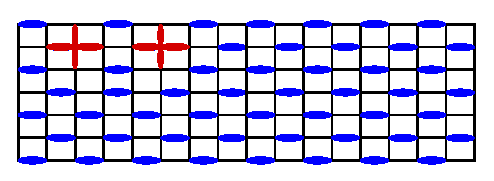
\includegraphics[width=8.5 cm]{ex_vert_mv_1}
    \caption{Step 1 in the vertical move example. Create a pair of stars.\label{fig:ex_vert_mv_1}}
\end{figure}

\begin{figure}[h]
    \centering
    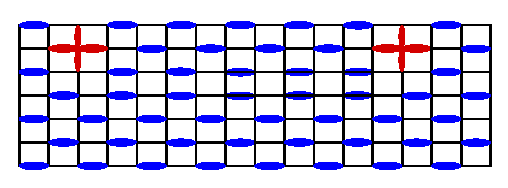
\includegraphics[width=8.5 cm]{ex_vert_mv_2}
    \caption{Step 2 in the vertical move example. Move the rightmost star right four times creating
    a horizontal set of flippable plaquettes.\label{fig:ex_vert_mv_2}}
\end{figure}

\begin{figure}[h]
    \centering
    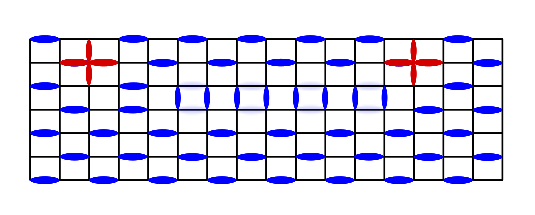
\includegraphics[width=8.5 cm]{ex_vert_mv_3}
    \caption{Step 3 in the vertical move example. Flip some of the plaquettes.\label{fig:ex_vert_mv_3}}
\end{figure}


\begin{figure}[h]
    \centering
    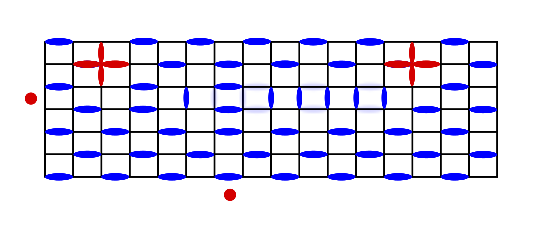
\includegraphics[width=8.5 cm]{ex_vert_mv_4}
    \caption{Step 4 in the vertical move example. Flip the plaquette at the $x$ and $y$ coordinates
    marked by the red dots.\label{fig:ex_vert_mv_4}}
\end{figure}


\begin{figure}[h]
    \centering
    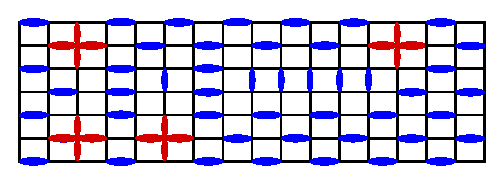
\includegraphics[width=8.5 cm]{ex_vert_mv_5}
    \caption{Step 5 in the vertical move example. Create another pair of stars.\label{fig:ex_vert_mv_5}}
\end{figure}

\begin{figure}[h]
    \centering
    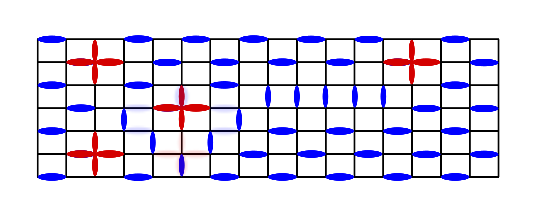
\includegraphics[width=8.5 cm]{ex_vert_mv_6}
    \caption{Step 6 in the vertical move example. Move the rightmost star of the new pair up.
    Rearrange the dimers around it to satisfy packing and conservation rules.\label{fig:ex_vert_mv_6}}
\end{figure}


% \bibliography{name_bib_file}

\end{document}
